\appendix
\chapter{Appendix}

%----------------------------------------------------------------------------------------
%	Section
%----------------------------------------------------------------------------------------

\section{Speech Signal Processing}

\subsection{Shelving Filter Design}
\label{shelving-appendix}
For gain $G$ in dB, center frequency of transition band $F_c$ in Hz and sampling frequency $F_s$, a high-frequency boost second-order shelving filter is represented by following equations as described in \cite{DAFX_book}.

\begin{equation}
y[n] = \frac{1}{a_0} \Big( b_0 x[n] + b_1 x[n-1] + b_2 x[n-3] - a_1 y[n-1] - a_2 y[n-2] \Big)
\end{equation}

\begin{align}
\begin{split}
b_0 &= \frac{V_0 + \sqrt{2V_0} K + K^2}{1 + \sqrt{2} K + K^2}\\
b_1 &= \frac{2 (K^2 - V_0)}{1 + \sqrt{2} K + K^2}\\
b_2 &= \frac{V_0 - \sqrt{2V_0} K + K^2}{1 + \sqrt{2} K + K^2}\\
a_1 &= \frac{2 (K^2 - 1)}{1 + \sqrt{2} K + K^2}\\
a_2 &= \frac{1 - \sqrt{2}K + K^2}{1 + \sqrt{2}K + K^2}
\end{split}
\end{align}
where $a_0 = 1$, $K = \tan(\pi F_c / F_s)$ and $V_0 = 10^{G/20}$.

%--------------------------------------------
%--------------------------------------------

\subsection{Mel-frequency Cepstral Coefficients Extraction}

Table \ref{table:frequency-mel-relationship} shows that $f[m]$ ($m = 0, 1, \dots, M+1$) are equally spaced in mel-scale where $f[0]$ = 0 Hz = 0 mel and $f[21]$ = 8000 Hz = 2835 mel.

\begin{table}[H]
\centering
\caption{Frequency and Mel-scale Relationship}
\label{table:frequency-mel-relationship}
\begin{tabular}{rrr|rrr}
\toprule
m &$f[m]$ in Hz &Mel-scale in mel &m &$f[m]$ in Hz &Mel-scale in mel\\
0  & 0      & 0    & 11 & 1920.4 & 1485\\
1  & 89.2   & 135  & 12 & 2254.5 & 1620\\
2  & 189.9  & 270  & 13 & 2631.2 & 1755\\
3  & 303.3  & 405  & 14 & 3055.9 & 1890\\
4  & 431.3  & 540  & 15 & 3534.7 & 2025\\
5  & 575.5  & 675  & 16 & 4074.7 & 2160\\
6  & 738.1  & 810  & 17 & 4683.4 & 2295\\
7  & 921.5  & 945  & 18 & 5369.8 & 2430\\
8  & 1128.2 & 1080 & 19 & 6143.7 & 2565\\
9  & 1361.3 & 1215 & 20 & 7016.2 & 2700\\
10 & 1624.1 & 1350 & 21 & 8000   & 2835\\
\bottomrule
\end{tabular}
\end{table}

%----------------------------------------------------------------------------------------
%	Section
%----------------------------------------------------------------------------------------

\section{Digital Signal Processor}

\subsection{Fixed-Point Data Types}

\begin{table}[H]
\centering
\caption{Fixed-Point Data Types}
\label{fixed-point-data-types}
\begin{tabu} to \textwidth {XXXX}
\toprule
Type &Size &Min &Max\\
\hline
\texttt{char} &8-bit &-128 &127\\
\hline
\texttt{unsigned char} &8-bit &0 &255\\
\hline
\texttt{short} &16-bit &-32,768 &32,767\\
\hline
\texttt{unsigned short} &16-bit &0 &65,535\\
\hline
\texttt{int} &32-bit &-2,147,483,648 &2,147,483,647\\
\hline
\texttt{unsigned int} &32-bit &0 &4,294,967,295\\
\hline
\texttt{long} &32-bit &-2,147,483,648 &2,147,483,647\\
\hline
\texttt{unsigned long} &32-bit &0 &4,294,967,295\\
\bottomrule
\end{tabu}
\end{table}

\subsection{Floating-Point Data Types}
\label{subsection:float-data-type}

\begin{figure}[H]
\begin{minipage}[t]{0.5\linewidth}
\centering
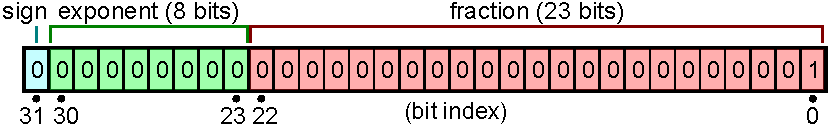
\includegraphics[width=\textwidth]{ang/smallest-denormalized-number}
\caption{Smallest Denormalized Number}
\label{ang/smallest-denormalized-number}
\end{minipage}
\begin{minipage}[t]{0.5\linewidth}
\centering
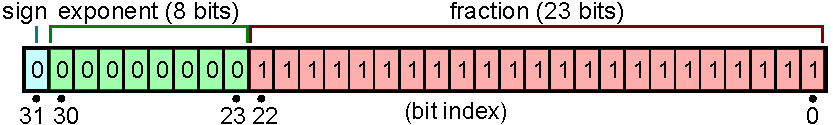
\includegraphics[width=\textwidth]{ang/largest-denormalized-number}
\caption{Largest Denormalized Number}
\label{ang/largest-denormalized-number}
\end{minipage}
\end{figure}

\begin{figure}[H]
\begin{minipage}[t]{0.5\linewidth}
\centering
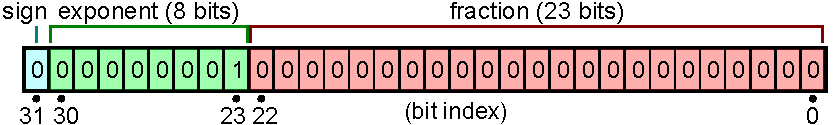
\includegraphics[width=\textwidth]{ang/smallest-normalized-number}
\caption{Smallest Normalized Number}
\label{ang/smallest-normalized-number}
\end{minipage}
\begin{minipage}[t]{0.5\linewidth}
\centering
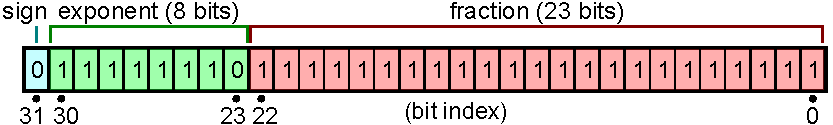
\includegraphics[width=\textwidth]{ang/largest-normalized-number}
\caption{Largest Normalized Number}
\label{ang/largest-normalized-number}
\end{minipage}
\end{figure}

Fig. \ref{ang/smallest-denormalized-number} to Fig. \ref{ang/largest-normalized-number} demonstrate the internal representation of a single-precision floating-point number. The actual mantissa (fraction part) includes 23 fraction bits to the right of the binary point and an \textit{implicit leading bit} to the left of the binary point. When the exponent part is equal to $(00000000)_2$, the implicit leading bit is with value 0 (denormalized); otherwise, the implicit leading bit takes 1 (normalized). Hence, the total length of mantissa is $(23 + 1)$ bits; in other words, \texttt{float} has a precision of $\log_{10}(2^{24}) \approx 7.225$ decimal digits.

\begin{align}
value &=
\begin{cases}
(-1)^{b_{31}} \times (0.b_{22}b_{21} \dots b_{0})_2 \times 2^{- 126} &\text{denormalized}\\
(-1)^{b_{31}} \times (1.b_{22}b_{21} \dots b_{0})_2 \times 2^{(b_{30}b_{29} \dots b_{23})_2 - 127} &\text{normalized}
\end{cases}\\
&=
\begin{cases}
\displaystyle(-1)^{b_{31}} \times \sum_{i=1}^{23} b_{23-i} 2^{-i} \times 2^{- 126} &\text{denormalized}\\
\displaystyle(-1)^{b_{31}} \times ( 1 + \sum_{i=1}^{23} b_{23-i} 2^{-i} ) \times 2^{\sum_{i=0}^{7} b_{i+23} 2^i - 127} &\text{normalized}
\end{cases}
\end{align}

\begin{table}[H]
\centering
\caption{Floating-Point Range}
\label{floating-point-range}
\begin{tabu} to \textwidth {XX}
\toprule
Number &Value\\
\hline
smallest denormalized number &$\pm 2^{-23} \times 2^{-126} \approx \pm 1.4 \times 10^{-45}$\\
\hline
largest denormalized number &$\pm (1-2^{-23}) \times 2^{-126} \approx \pm 1.18 \times 10^{-38}$\\
\hline
smallest normalized number &$\pm 1 \times 2^{-126} \approx \pm 1.18 \times 10^{-38}$\\
\hline
largest normalized number &$\pm (2-2^{-23}) \times 2^{127} \approx \pm 3.4 \times 10^{38}$\\
\bottomrule
\end{tabu}
\end{table}

%----------------------------------------------------------------------------------------
%	Section
%----------------------------------------------------------------------------------------

\section{Design and performance}

\begin{longtable}[c]{|c|c|c|}
\caption {Accuracy of Speaker Dependent System and Speaker Independent System\label{table 3}}\\

\hline
Word & Speaker Dependent System  & Speaker Independent System \\
\hline
\endfirsthead

\hline
Word & Speaker Dependent System  & Speaker Independent System \\
\hline
\endhead

\hline
\endfoot

\hline
\endlastfoot

1& 1 & 0.6\\
\hline
2& 1 &  0.3\\
\hline
3& 1&  0.7\\
\hline
4& 1& 0.3\\
\hline
5& 1& 0.4\\
\hline
6& 1 &  0.6 \\
\hline
7& 1 &   0.2\\
\hline
8& 0.9 &   0.7\\
\hline
9&1 &   0.5\\
\hline
10&1 &  0.8\\
\hline
11& 1 &  0.4\\
\hline
12& 1 &   0.4\\
\hline
13& 1 &   0.5\\
\hline
14& 0.9 & 0.5\\
\hline
15& 1 &  0.3 \\
\hline
16& 1 &  0.5 \\
\hline
17& 1 &  0.2\\
\hline
18& 1 &   0.2\\
\hline
19&0.9& 0.1\\
\hline
20&1 &   0.3\\
\hline
21&1 &  0.5\\
\hline
22& 1 &  0.3\\
\hline
23& 1 &  0.6\\
\hline
24& 1 &   0.4\\
\hline
25& 1 &   0.7\\
\hline
26& 1 &  0.1\\
\hline
27& 0.9 &  0\\
\hline
average & 98.52\% & 41.11\% \\
\end{longtable}


\begin{longtable}[c]{|c|c|c|c|}
\caption{Accuracy of different training data number\label{table 2}}\\

\hline
Word & $\#$ of training data = 20 &$\#$ of training data = 35 &$\#$ of training data = 50 \\
\hline
\endfirsthead

\hline
Word & $\#$ of training data = 20 &$\#$ of training data = 35 &$\#$ of training data = 50 \\
\hline
\endhead

\hline
\endfoot

\hline
\endlastfoot

1& 0.5&0.89 &0.81 \\
\hline
2& 0.5&0.41 &0.60 \\
\hline
3& 0.45& 0.75&0.96 \\
\hline
4& 0.4&0.69 &0.86 \\
\hline
5& 0.5& 0.61& 0.88\\
\hline
6& 0.75& 0.96 &0.96 \\
\hline
7& 0.6&0.62 &0.83 \\
\hline
8& 0.85&0.88 &0.92 \\
\hline
9& 0.35&0.42 &0.60 \\
\hline
10& 0.8& 0.75& 0.91\\
\hline
11& 0.45& 0.58& 0.81\\
\hline
12& 0.55& 0.79&0.88 \\
\hline
13& 0.4&0.38 &0.44 \\
\hline
14& 0.55&0.86 &0.78 \\
\hline
15& 0.4& 0.65&0.70 \\
\hline
16& 0.45&0.48 &0.65 \\
\hline
17& 0.3& 0.31& 0.47\\
\hline
18& 0.2& 0.38&0.78 \\
\hline
19& 0.2& 0.21&0.57 \\
\hline
20& 0.85& 0.79&0.94 \\
\hline
21& 0.6& 0.72& 0.91\\
\hline
22& 0.3& 0.62& 0.57\\
\hline
23& 0.75&0.65 &0.78 \\
\hline
24& 0.55& 0.75&0.81 \\
\hline
25& 0.95&0.98 &0.96 \\
\hline
26& 0.05& 0.24& 0.52\\
\hline
27& 0& 0.08& 0.10\\
\hline
average & 49.07\% & 60.90\% & 74.08\% \\
\end{longtable}

%----------------------------------------------------------------------------------------
%	Section
%----------------------------------------------------------------------------------------

\section{Final Implementation}

\begin{figure}[H]
\centering
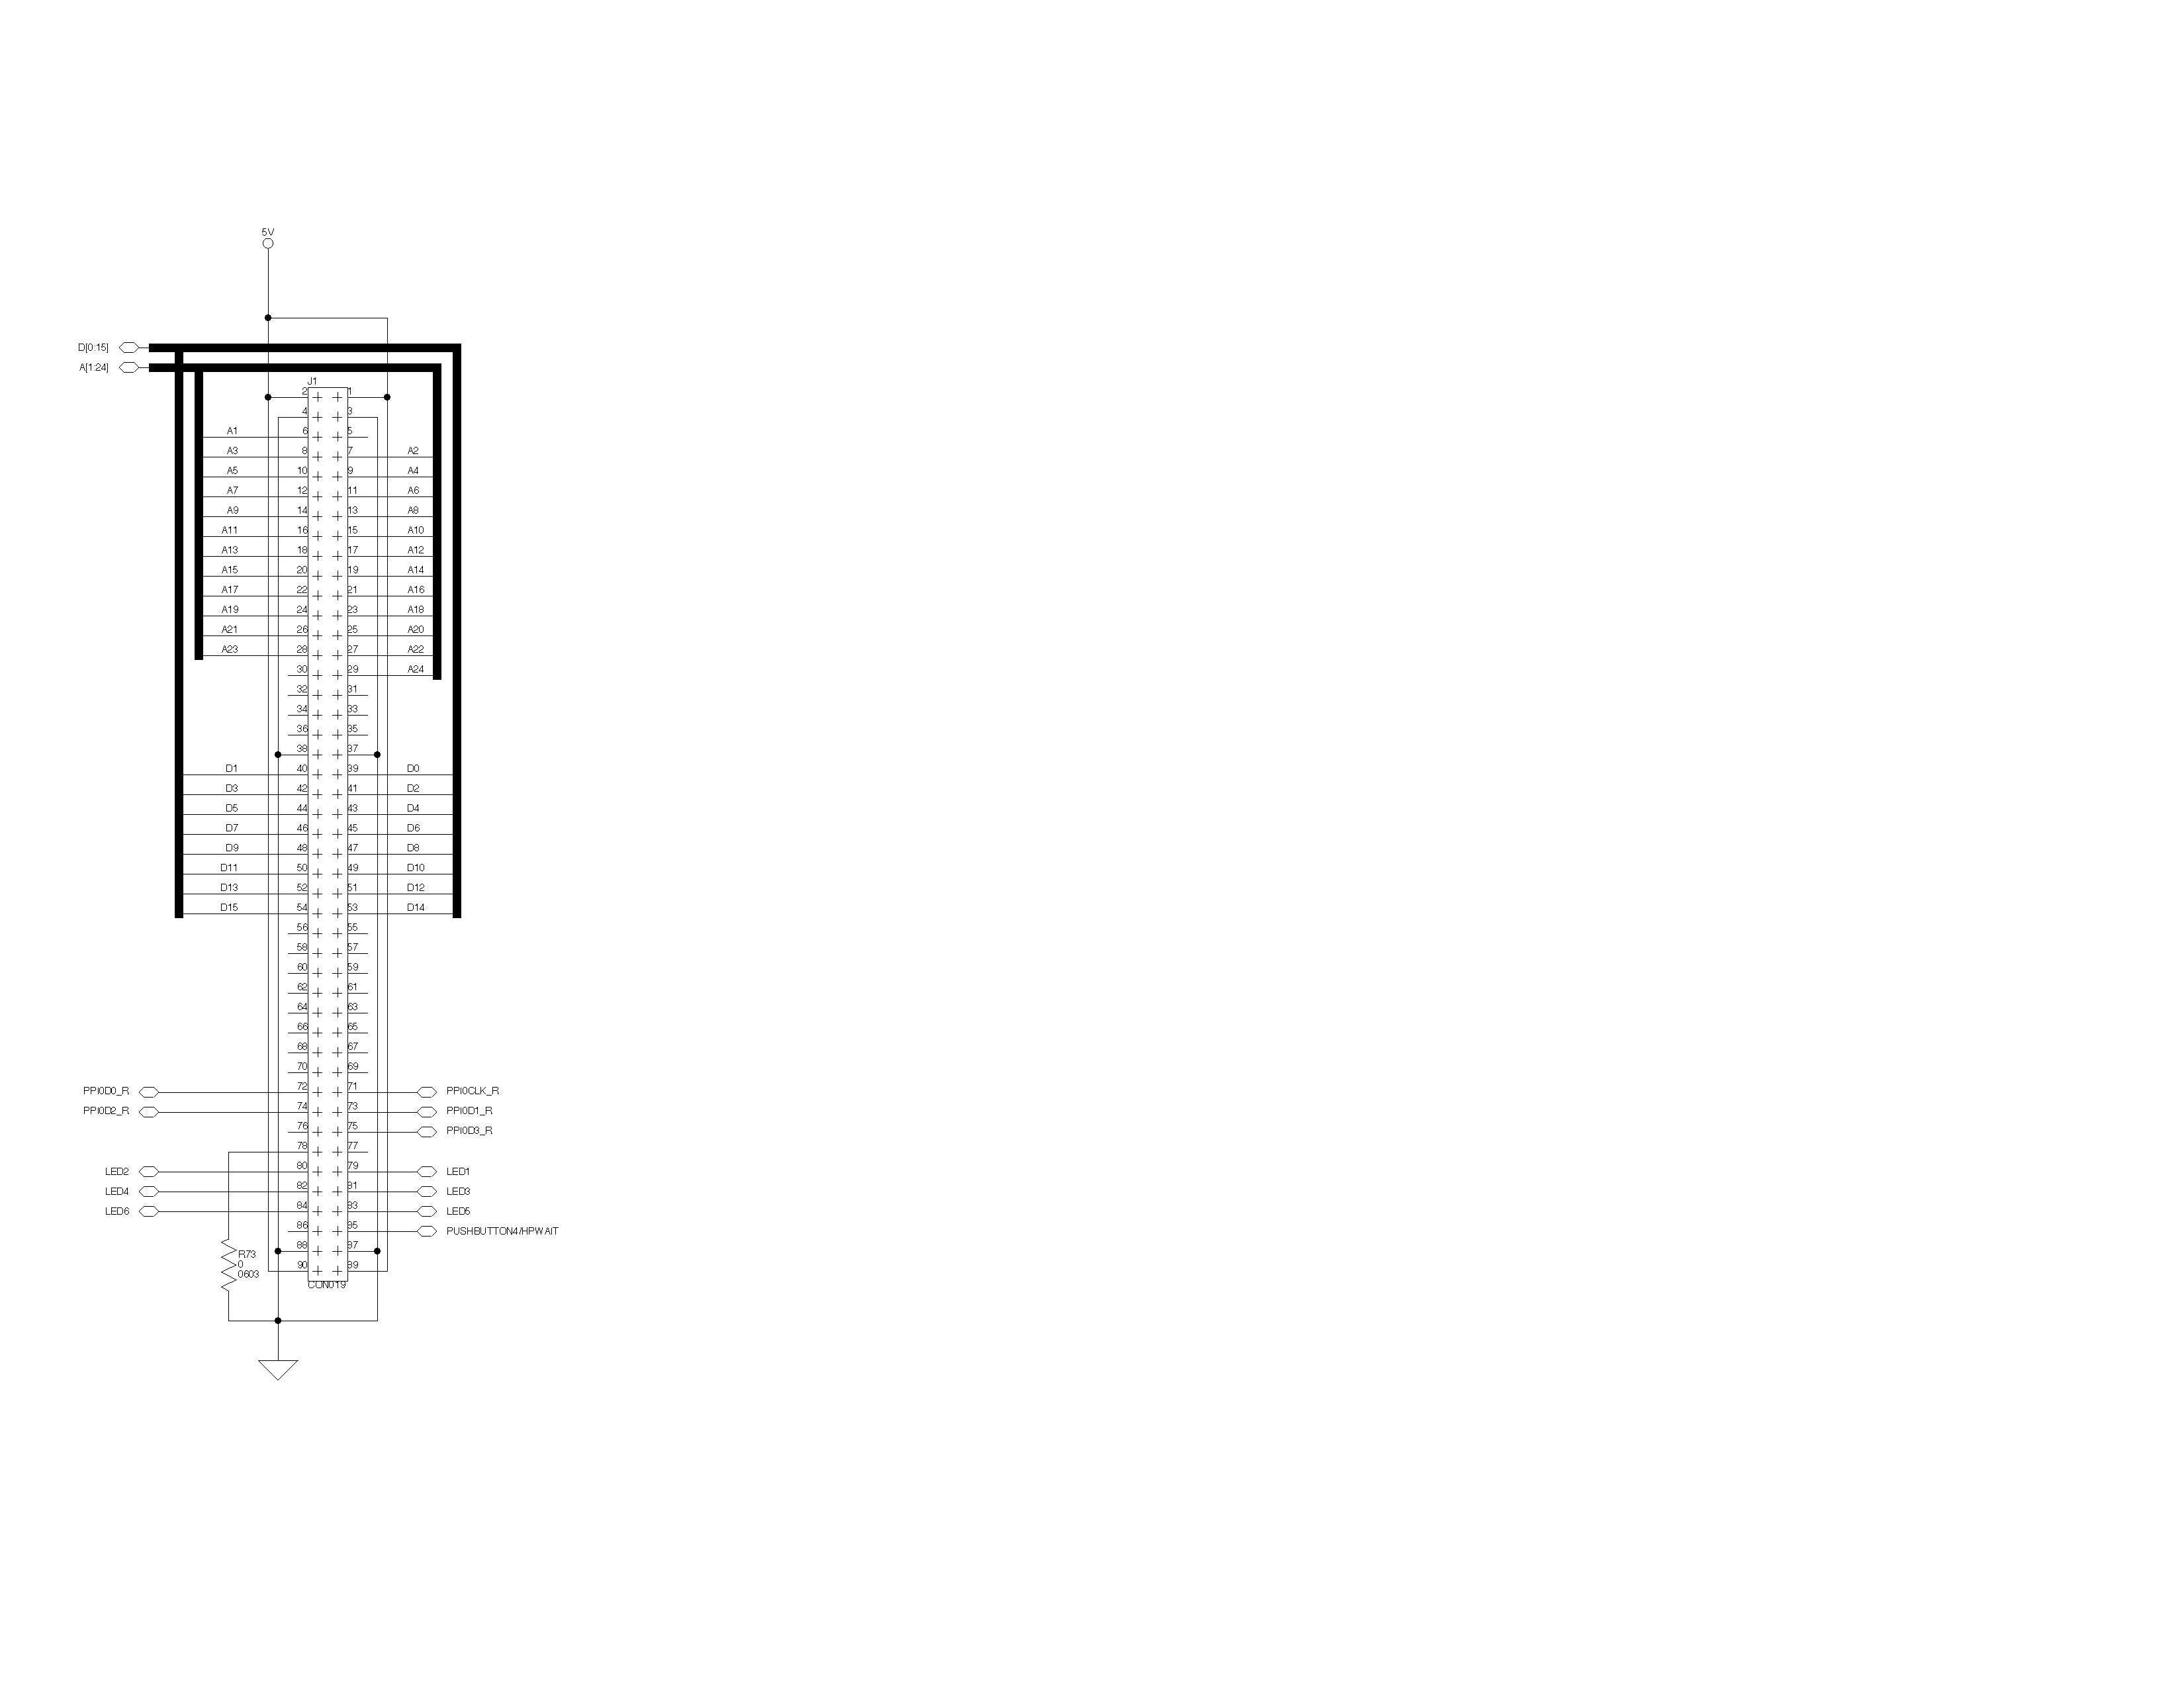
\includegraphics[width=3in]{ang/J1-schematic}
\caption{ADSP-BF548 J1 Connector \cite{bf548-manual}}
\label{J1-schematic}
\end{figure}
